\section{Afprøvning}

\subsection{Hvordan vil vi vurdere resultatet}

\todo{Beskriv joint histogram + mere}

\subsection{Planlagte forsøg}
\todo{Renskriv, mere tekst, omdøb faldgrupper}

\subsubsection{Leave-one-out cross validation (LOOCV)}
\paragraph{Fremgangsmåde}
Tag 5 hjerner. Træn på 4 og test på 1 og roter.

\todo{Uddyb}

\paragraph{Forventning}
Vi forventer, at vores joint histogram bliver nogenlunde lineær. 

\paragraph{Faldgrupper}
Billeder med artifakter kan forstyrre algoritmen. 

\paragraph{Resultat}
\todo{Udfør LOOCV-forsøget}

\begin{figure}
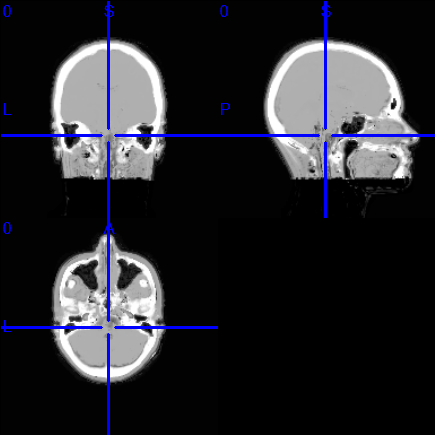
\includegraphics[width=\linewidth]{sct0.png}
\caption{sct0.png}
\end{figure}

\begin{figure}
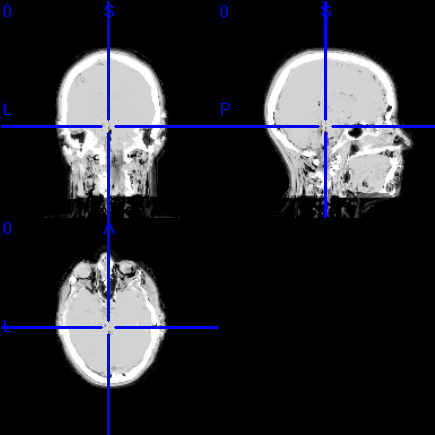
\includegraphics[width=\linewidth]{sct1.png}
\caption{sct1.png}
\end{figure}

\begin{figure}
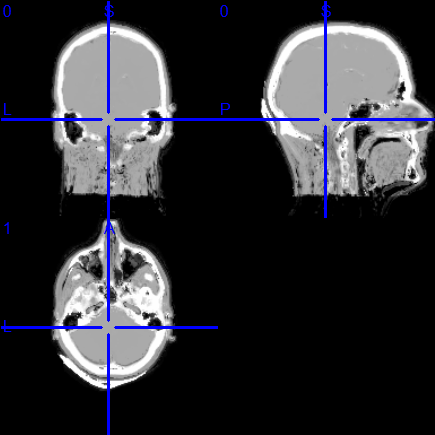
\includegraphics[width=\linewidth]{sct5.png}
\caption{sct5.png}
\end{figure}

\subsubsection{Udregn sCT til hjerner med artifakter trænet på hjerner uden artifakter}
\paragraph{Fremgangsmåde}
Træn på n hjerner test på m.

\paragraph{Forventning}

\paragraph{Faldgrupper}

\paragraph{Resultat}

\subsubsection{Udregn sCT til hjerner trænet på hjerner med artifakter}
\paragraph{Fremgangsmåde}
Iterativt træn på et antal hjerner og introducer hjerner med artifakter.
Sammenlign kvaliteten af sCT afhængigt af andelen af hjerner, som har
artifakter.

\paragraph{Forventning}
At sCT's kvalitet forværes for hver introduceret hjerne med artifakt.

\paragraph{Faldgrupper}

\paragraph{Resultat}


\subsubsection{Over tid}
\paragraph{Fremgangsmåde}
Træn på gamle hjerner, test på ny hjerner. Og omvendt.

\paragraph{Forventning}
Forventningen er sCT af samme kvalitet, som dem ved LOOCV-forsøget.

\paragraph{Faldgrupper}


\paragraph{Resultat}

\subsubsection{Test på en masse}
\paragraph{Fremgangsmåde}
Iterativt træn på n+1 hjerner

\paragraph{Forventning}
Forventning er at efter 7-8 hjerner giver det ikke rigtig nogen
kvalitetsforskel.

\paragraph{Faldgrupper}
Overfitting. 


\paragraph{Resultat}

\subsubsection{Hvorfor 20-gaussians?}

\paragraph{Fremgangsmåde}
Test på forskelligt antal gaussians og sammenlign resultaterne.

\paragraph{Forventning}
Vi forventer, at kvaliteten falder under 20, men at metoden kræver mere tid
efter 20 uden betydelig forbedringer.

\paragraph{Faldgrupper}
Overfitting. 

\paragraph{Resultat}



\subsection{Test og vurdering af sCT}

\todolasse{Vi mangler at teste sCT}
\todolasse{Vi har ikke vurderet sCT}

\subsection{Test og vurdering af sCT - FullCT}

\todolasse{Vi mangler at teste sCT ved brug i FullCT}
\todolasse{Vi har ikke vurderet sCT ved brug i FullCT}

\subsection{Sammenligning med standard CT og FullCT}

\todolasse{Sammenligning med standard CT mangler}
